\documentclass[11pt]{report}
\usepackage{eso-pic,graphicx}
\usepackage[export]{adjustbox}
\usepackage{url}
\usepackage[top=2cm, bottom=2cm, outer=2cm, inner=2cm]{geometry}
\begin{document}
\AddToShipoutPictureBG*{
\includegraphics[width=\paperwidth,height=\paperheight]{images/bkgrnd}}
\begin{center}
\vspace*{2cm}
\textsf{\begin{Huge}
\textbf{ELP­718 ­ Telecom Software Laboratory \\
1st Semester, 2016-18 \\
Abhishek Mishra\\
23 Aug 2016, 5pm\\
Assignment-5}\\
\end{Huge}}
\vspace*{6cm}

\includegraphics[scale=0.12, center]{images/iitlogo}
\end{center}
\pagebreak
\tableofcontents
\vspace{5cm}
\pagebreak
\section{Introduction}
\vspace*{1cm}
This assignment aims to provide a better understanding of the following topics:\\

\begin{flushleft}
1. \textbf{Shell Scripting}\\
A shell script is a computer program designed to be run by the Unix shell, a command-line interpreter. The various dialects of shell scripts are considered to be scripting languages.The typical Unix/Linux/Posix-compliant installation includes the Korn Shell (ksh) in several possible versions such as ksh88, Korn Shell '93 and others.\\
The oldest shell still in common use is the Bourne shell (sh); Unix systems invariably include also the C Shell (csh), Bourne Again Shell (bash), a remote shell (rsh), a secure shell for SSL telnet connections (ssh), and a shell which is a main component of the Tcl/Tk installation usually called tclsh; wish is a GUI-based Tcl/Tk shell. The C and Tcl shells have syntax quite similar to that of said programming languages, and the Korn shells and Bash are developments of the Bourne shell, which is based on the ALGOL language with elements of a number of others added as well.\\
On the other hand, the various shells plus tools like awk, sed, grep, and BASIC, Lisp, C and so forth contributed to the Perl programming language\\
\end{flushleft}

\begin{flushleft}
2. \textbf{Vim Editor}\\
 
Vim (Vi IMproved) is a clone of Bill Joy's vi text editor program for Unix. It was written by Bram Moolenaar based on source for a port of the Stevie editor to the Amiga and first released publicly in 1991.\\
Vim is designed for use both from a command-line interface and as a standalone application in a graphical user interface. Vim is free and open source software and is released under a license that includes some charityware clauses, encouraging users who enjoy the software to consider donating to children in Uganda. The license is compatible with the GNU General Public License.\\
\end{flushleft}
\newpage
\section{Problem Statement 1}
	This problem requires us to take input through command line argument from the user and then process it similar to following outputs:\\
	\begin{figure}[h!]
	\centering
	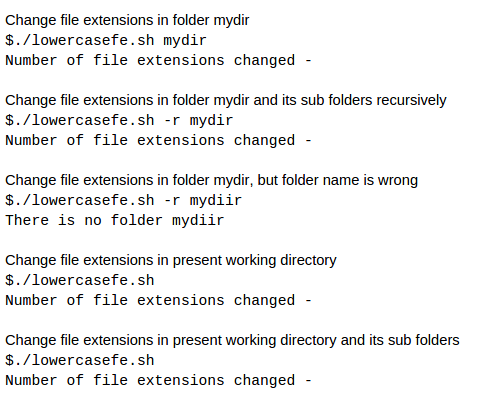
\includegraphics[scale=0.7]{images/Selection_003}	
	\end{figure}
	\subsection{Assumptions}
	The user shall input either no name to a directory or he will enter an existing directory.
	\pagebreak
	\subsection{Structure Chart and Implementation}
	\begin{figure}[h!]
	\centering
	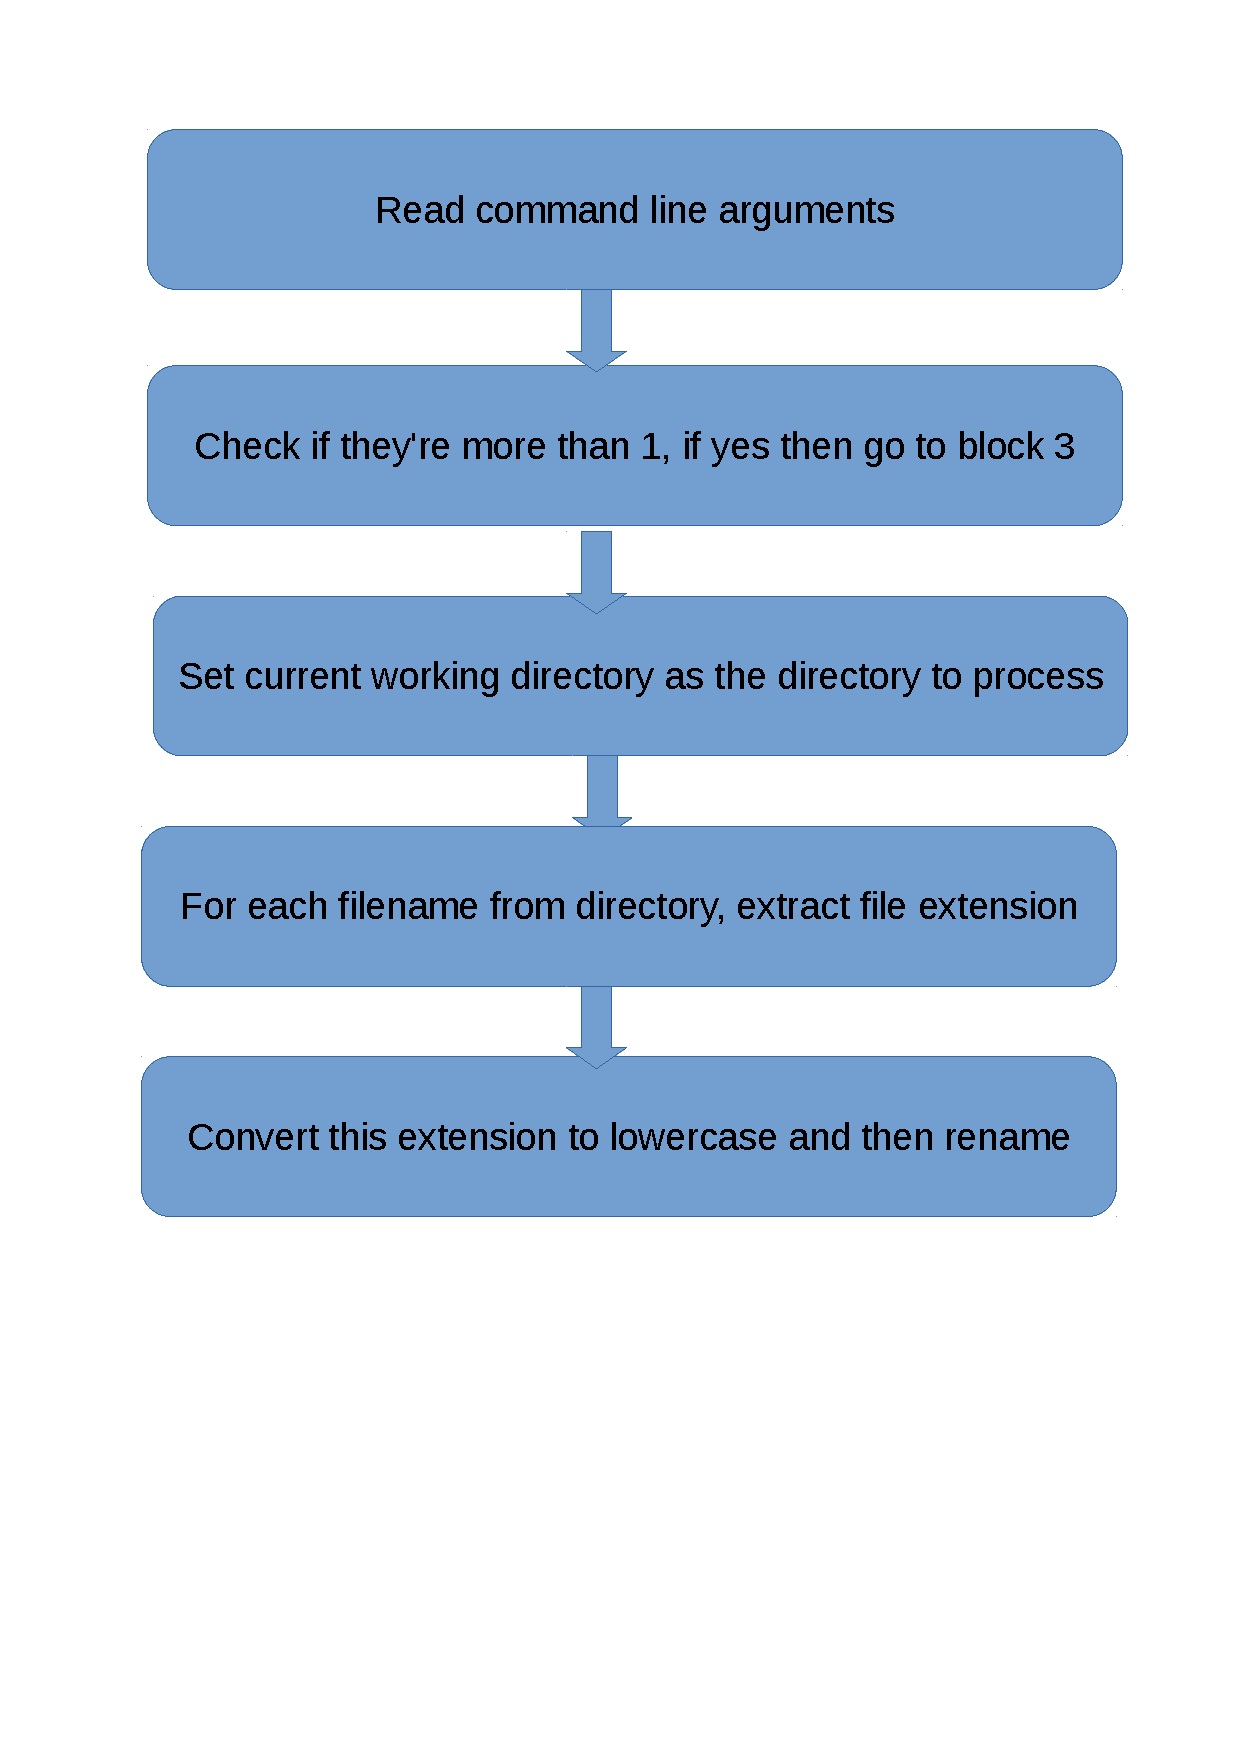
\includegraphics[scale=0.7]{images/shots11}
	\caption{Structure chart for problem 1}
	\end{figure}		
	\pagebreak
	\subsection{Screenshots}
	\begin{figure}[h!]
	\centering
	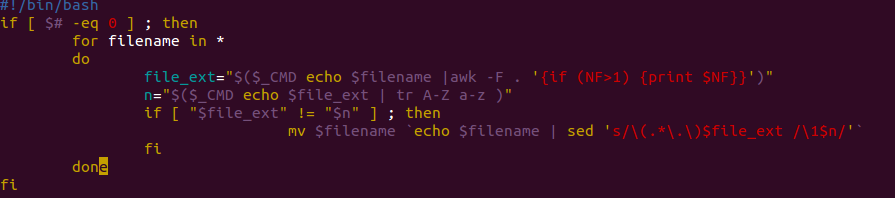
\includegraphics[scale=0.8, center]{images/screenshot1}
	\caption{Screenshot for problem statement 1}
	\end{figure}
	\pagebreak
\section{Problem Statement 2}
	The problem requires you to display system information in the following manner. \\
	\begin{figure}[h!]
	\centering
	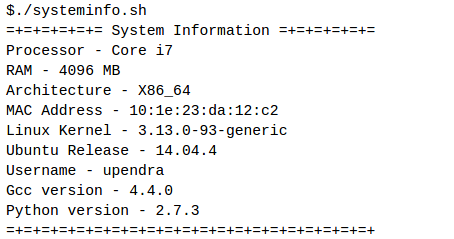
\includegraphics[scale=0.7]{images/Selection_001}	
	\end{figure}
	\subsection{Assumptions}
	The output is to be processed in the exact manner as shown in the image
	\pagebreak
	\subsection{Structure Chart}
	\begin{figure}[h!]
	\centering
	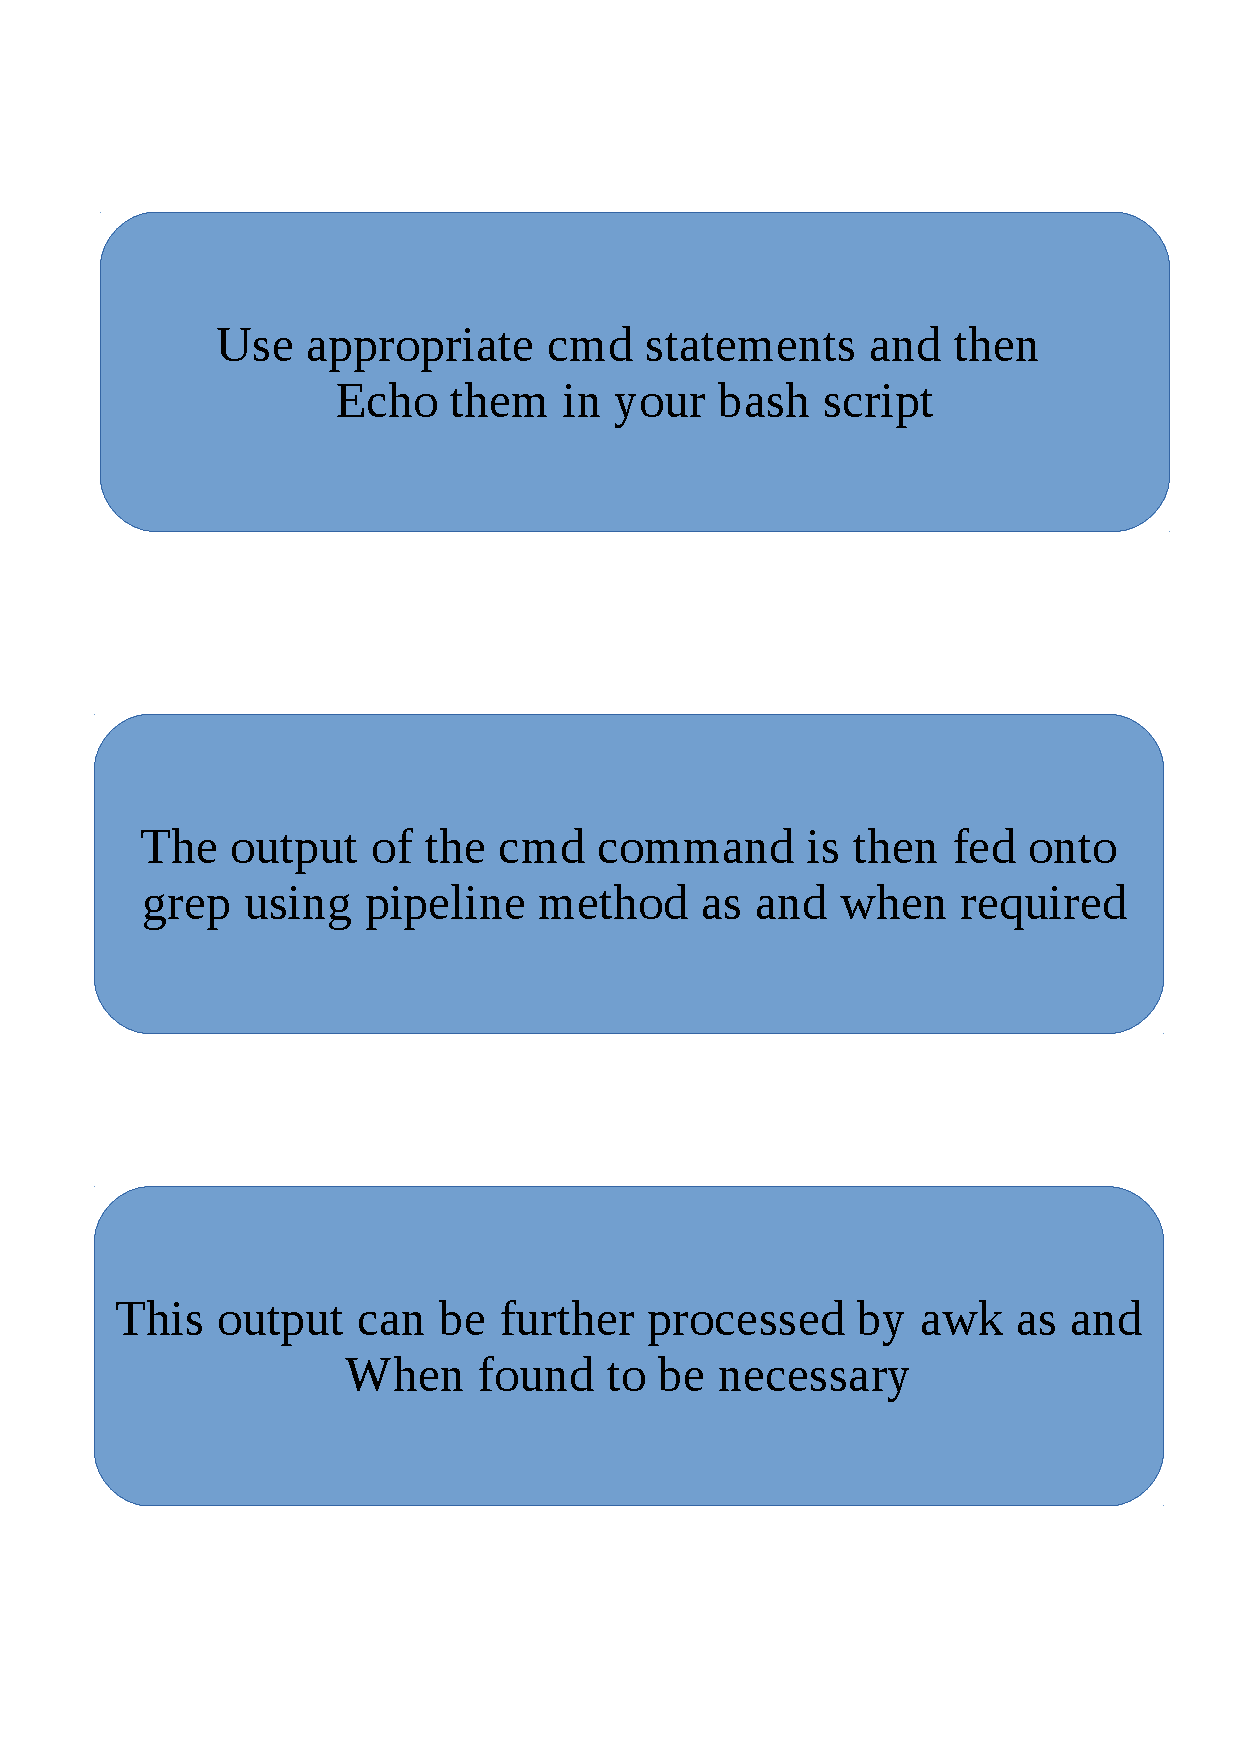
\includegraphics[scale=0.7]{images/shots22}
	\caption{Structure chart for problem 2}	
	\end{figure}
	\pagebreak
	\subsection{Screenshots}
	\begin{figure}[h!]
	\centering
	
\includegraphics[scale=0.8, center]{images/screenshot2}
	\caption{Screenshot for problem statement 2}
	\end{figure}
	\pagebreak
\section{Problem Statement 3}
\textbf{Part - 1 -}\\
Write shell script to emulate behaviour of bash, but also record every command put up on terminal on a logger.txt file along with time stamp. Your command prompt should look like normal bash command prompt. \\
	\subsection{Assumptions}
	The output is to be processed in the exact manner as shown in the image\\
	\begin{figure}[h!]
	\centering
	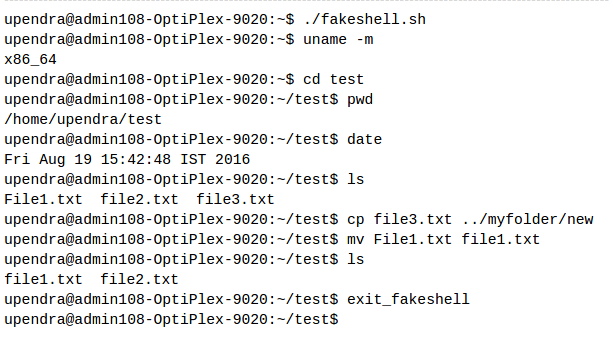
\includegraphics[scale=0.7]{images/Selection_004}	
	\end{figure}
	\pagebreak
	\subsection{Structure Chart}
	\begin{figure}[h!]
	\centering
	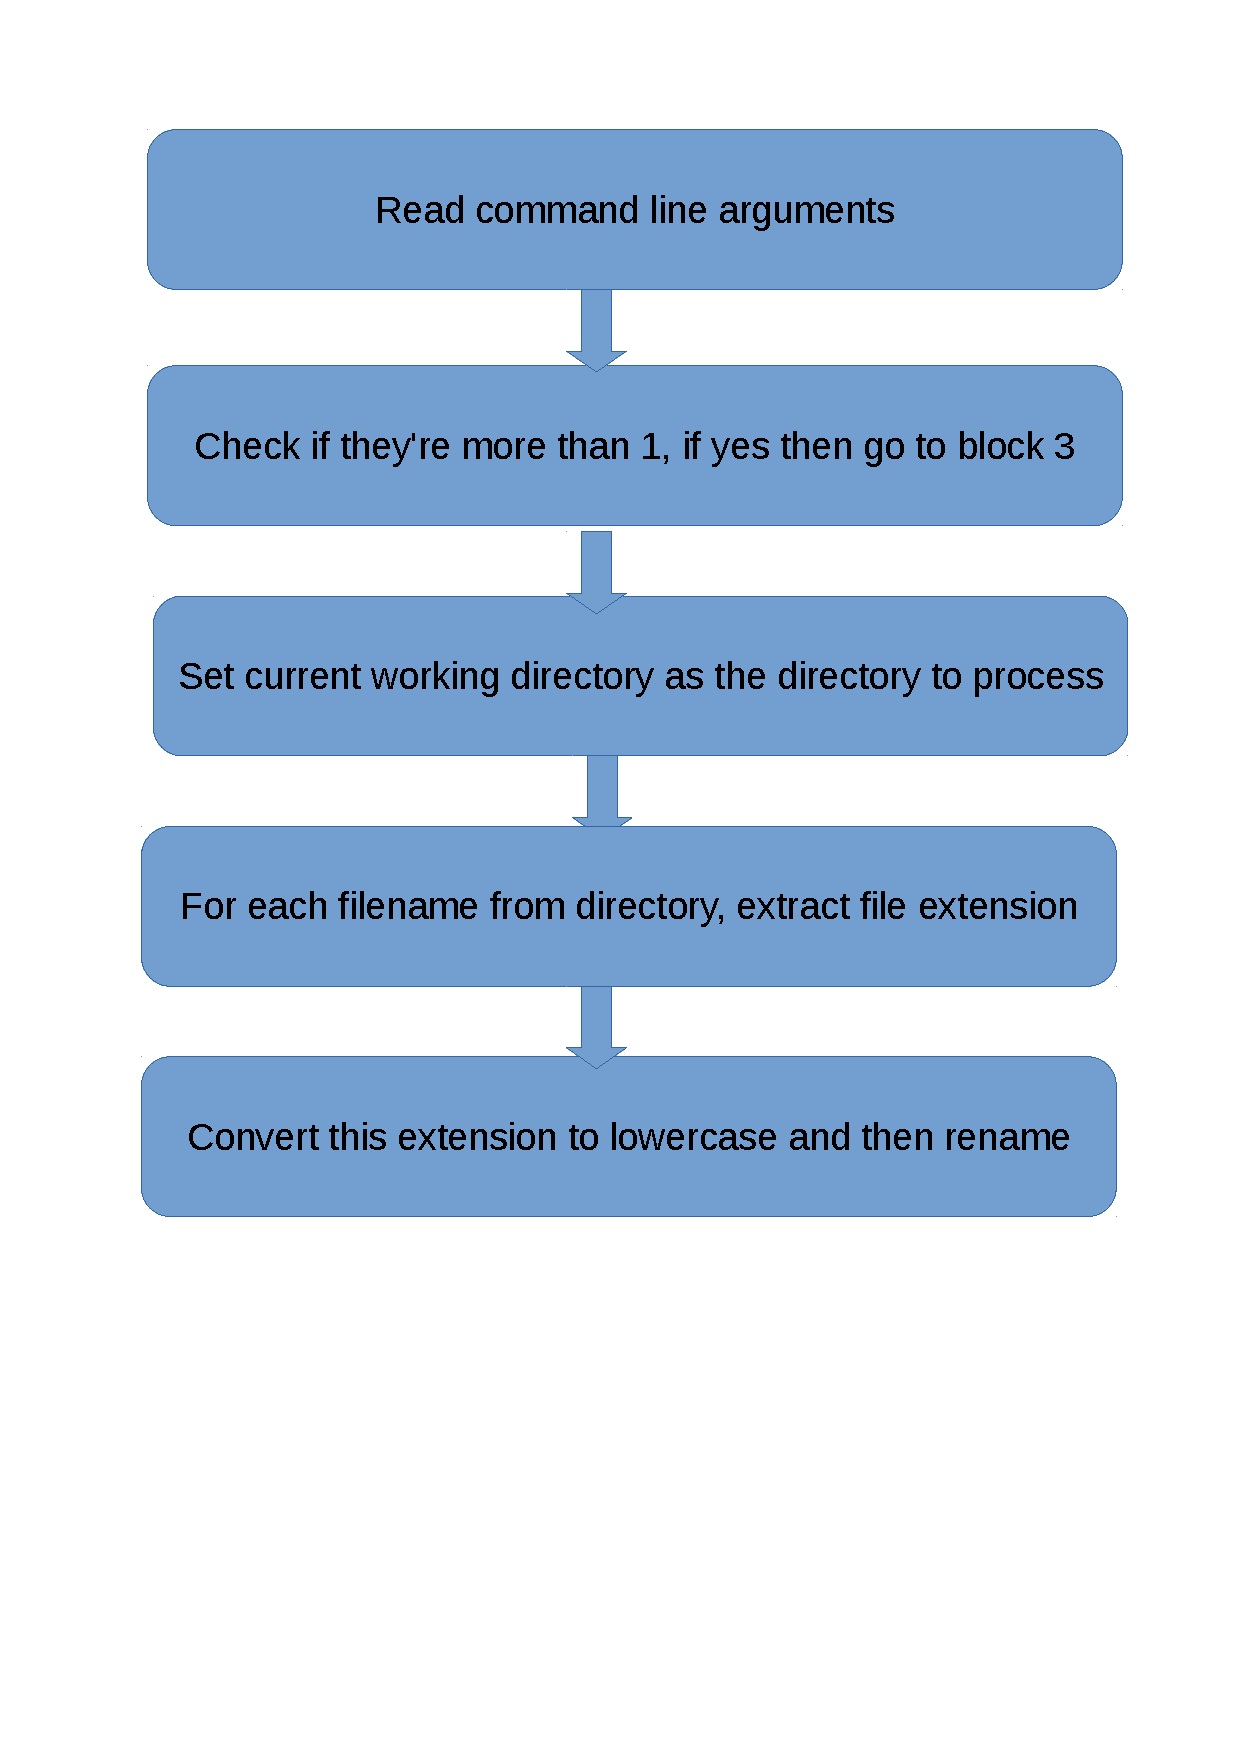
\includegraphics[scale=0.7]{images/shots33}
	\caption{Structure chart for problem 3}	
	\end{figure}
	\pagebreak
\section{Epilogue}
The execution of the first problem involved me to break it down and then try to figure out solution to each and every part of it. To some extent I feel I have been successful in justifying the problem.\\
Whereas for problem statement 2, it was a different but not so difficult problem statement compared to problem 1. \\
Then i found the problem 3 to be the toughest of all problems.\\
This week's assignment too has taught me a lot of things on which I shall further improve upon in the next assignment.\\
\bibliography{biblio} 
\bibliographystyle{ieeetr}
\nocite{*}
\end{document}